\section{System Overview}
\label{sec:system}
\textsc{Rivulet} is implemented on top of Neptune stream processing system~\cite{buddhika2016neptune} as a specialized layer for geo-spatial data.
In this section, we will briefly introduce Neptune followed by a discussion on the design of Rivulet.

\subsection{Neptune}
Neptune is a distributed stream processing system which is optimized to process high throughput data streams.
It is designed to cope with application requirements such as high volumes of small stream packets, high and variable data rates and heterogeneity within stream processing jobs.
Satisfying these requirements imposes various system level challenges including possible buffer-overflow errors, increased number of context-switches, object creation overhead and memory management issues.
Neptune takes a holistic approach that considers CPU, memory, network and kernel issues to address the above challenges.
This is achieved through employing a set of optimizations such as application level buffering, batched scheduling, object re-use, built-in support for backpressure and selective compression to ensure a better utilization of system resources.

Users can deploy stream processing jobs as directed acyclic graphs in Neptune.
A stream processing graph consists of a set of stream ingestion points and stream processors (vertices) and streams connecting these operators (edges).
To provide each job with a initial load-balanced deployment plan to start with, each operator in a stream processing graph can be annoated with a parallelism level while each stream can be associated with a partitioning scheme.

\begin{figure}
    \centerline{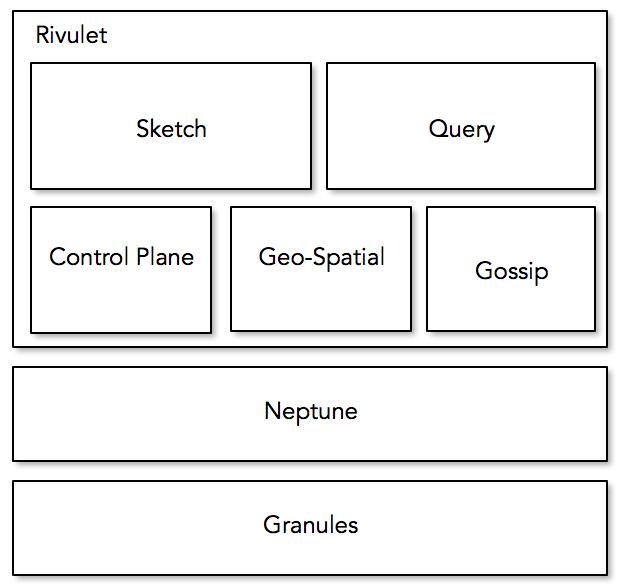
\includegraphics[scale=0.5]{figures/rivulet-archi.png}}
    \caption{Rivulet is implemented as a specialized layer for geo-spatial data on top of Neptune stream processing system..}
    \label{fig:process-monitor}
\end{figure}
%
\begin{figure}
    \centerline{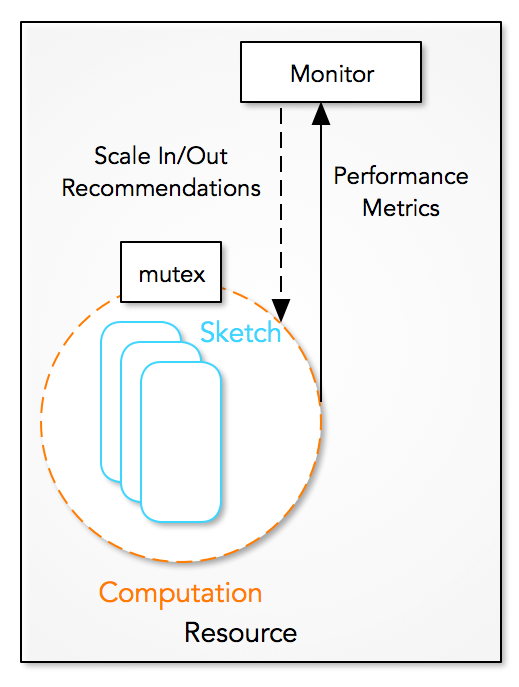
\includegraphics[scale=0.55]{figures/process-monitor.png}}
    \caption{Dynamic scaling is triggered by monitoring the backlog of each computation and memory pressure incurred in each process.}
    \label{fig:process-monitor}
\end{figure}